\section{Definição Geométrica}

Napier também desenvolveu uma definição geométrica para o logaritmo. 
Considere um segmento de reta $AB$ e uma semirreta $DE$, de origem $D$, conforme a figura \ref{fig:defgeolog}. 
Suponhamos que os pontos $C$ e $F$ se ponham em movimento simultaneamente a partir de $A$ e $D$, respectivamente, 
ao longo dessas linhas, com a mesma velocidade inicial. 
Admitamos que $C$ se mova com uma velocidade numericamente sempre igual à distância $CB$, 
e que $F$ se mova com velocidade uniforme. 

\begin{figure}[h!]
    \centering
    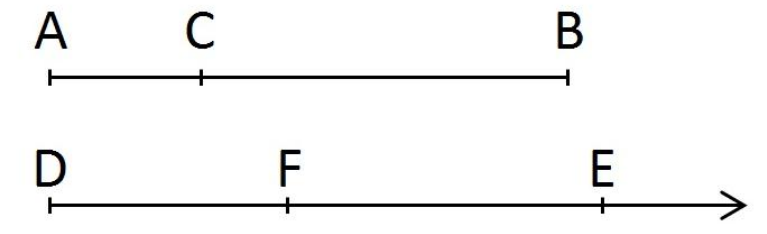
\includegraphics[width=0.4\linewidth]{img/defgeo.png}
    \caption{Definição Geométrica de logaritmo}
    \label{fig:defgeolog}
\end{figure}

Napier definiu então $DF$ como logaritmo de $CB$. 
Isto é, pondo $DF = x$ e $CB = y$, temos:

\[
x = \text{Naplog}\, y
\]

Para demonstrar esse fato, utilizaremos ferramentas do cálculo diferencial e integral que temos atualmente. Tomando $AB = 10^7$, $x=DF$, $y = CB$, sabemos que a velocidade de $C$ é a derivada de seu deslocamento, ou seja, temos que:

\[
\dfrac{d}{dt}(10^7 - y) = y \iff -\dfrac{dy}{dt} = y
\]

Resolvendo essa equação diferencial, temos que $y(t) = Ce^{-t}$, como $y(0) = C = 10^7$, segue que:

\[
y(t) = 10^7 e^{-t}
\]

Além disso, como $x(t)$ tem velocidade constante, $x(t)= 10^7 t$. Daí, obtemos as seguintes funções de deslocamento:

\[
y(t) = 10^7 e^{-t} \qquad \text{e} \qquad x(t)= 10^7 t
\]

Portanto, obtemos que:

\[
x = 10^7 t = 10^7 \cdot \text{ln}\left(\frac{10^7}{y}\right)
\]

Observe que as definições não coincidem exatamente, mas como Napier tomou $10^7$, isto é, um número muito grande. As definições são aproximadamente equivalentes. De fato, após algumas manipulações algébricas e utilizando que $\text{ln}\left(1-\frac{1}{10^7}\right) \approx -\frac{1}{10^7}$, conseguimos obter que:

\[
y = 10^7 (1-10^{-7})^{x} \implies x \approx 10^7 \text{ln}\left(\frac{10^7}{y}\right)
\]

Para visualizar essa definição geométrica, fizemos uma construção geométrica no \textit{geogebra}. Para melhor visualização utilizamos $AB = 10$. O ponto $P$ desliza sobre o plano $\mathbb{R}^2$ de modo que $P = (CB(t), DF(t))$, assim, conseguimos visualizar que isso constrói um gráfico de uma função logarítimica.

Abaixo segue o link para interação com o programa: https://www.geogebra.org/classic/hjcec98z

